\documentclass[tikz, border=15pt]{standalone}
\usetikzlibrary{positioning, arrows.meta}

\usepackage[T1]{fontenc}
\usepackage[utf8]{inputenc}
\usepackage{textcomp}
\renewcommand{\ttdefault}{lmtt}

\begin{document}
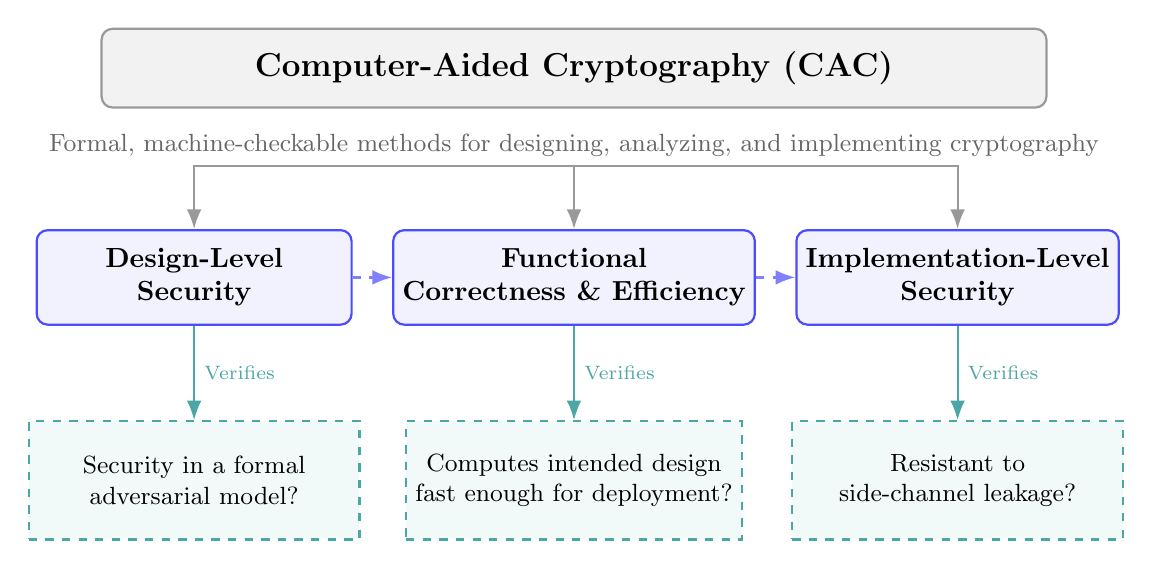
\begin{tikzpicture}[
	>=stealth,
	font=\sffamily,
	% Define styles
	titlebox/.style={rectangle, draw=gray!80, fill=gray!10, rounded corners, thick, minimum width=12cm, minimum height=1cm, font=\large\bfseries},
	layer/.style={rectangle, draw=blue!70, fill=blue!5, rounded corners, thick, minimum width=4cm, minimum height=1.2cm, align=center, font=\bfseries},
	question/.style={rectangle, draw=teal!70, fill=teal!5, thick, dashed, minimum width=4.2cm, minimum height=1.5cm, align=center, font=\small},
	takeaway/.style={rectangle, draw=orange!80, fill=orange!5, rounded corners, thick, text width=12.5cm, align=center, inner sep=10pt},
	arrow/.style={-{Latex[length=2.5mm]}, thick, gray!80},
	checkarrow/.style={-{Latex[length=2.5mm]}, thick, teal!70}
	]
	
	% 1. Main Subject
	\node[titlebox] (main) {Computer-Aided Cryptography (CAC)};
	
	% Subtext
	\node[below=0.2cm of main, font=\small\color{gray!80!black}] (subtitle) {
		Formal, machine-checkable methods for designing, analyzing, and implementing cryptography
	};
	
	% 2. Cryptographic Assurance Layers
	\node[layer, below=0.8cm of subtitle] (correctness) {Functional\\Correctness \& Efficiency};
	\node[layer, left=0.5cm of correctness] (design) {Design-Level\\Security};
	\node[layer, right=0.5cm of correctness] (implsec) {Implementation-Level\\Security};
	
	% Structural arrows for layers connecting from the top
	\draw[arrow] (subtitle.south) -| (design.north);
	\draw[arrow] (subtitle.south) -- (correctness.north);
	\draw[arrow] (subtitle.south) -| (implsec.north);
	
	% Process flow arrows between layers
	\draw[arrow, blue!50, dashed] (design) -- (correctness);
	\draw[arrow, blue!50, dashed] (correctness) -- (implsec);
	
	% 3. Core Questions / Checks
	\node[question, below=1.2cm of design] (qdesign) {Security in a formal\\adversarial model?};
	\node[question, below=1.2cm of correctness] (qcorrect) {Computes intended design\\fast enough for deployment?};
	\node[question, below=1.2cm of implsec] (qimplsec) {Resistant to \\side-channel leakage?};
	
	% 4. Check arrows
	\draw[checkarrow] (design.south) -- (qdesign.north) node[midway, right, font=\scriptsize\color{teal!70}, align=left] {Verifies};
	\draw[checkarrow] (correctness.south) -- (qcorrect.north) node[midway, right, font=\scriptsize\color{teal!70}, align=left] {Verifies};
	\draw[checkarrow] (implsec.south) -- (qimplsec.north) node[midway, right, font=\scriptsize\color{teal!70}, align=left] {Verifies};
	
%	% 5. Takeaway Footer
%	\node[takeaway, below=1.5cm of qcorrect] (footer) {
%			No single tool solves all layers. CAC relies on a \textbf{collection of tool families} that 
%		integrate to provide high-assurance cryptographic systems.
%%		\textbf{The Assurance Ecosystem:}\\
%%		No single tool solves all three layers. The field relies on a \textbf{collection of tool families}\\
%%		with different strengths that fit together to give stronger assurance for cryptographic systems.
%	};
%	
%	% Connecting questions to the footer to show integration
%	\draw[arrow, orange!80, dashed] (qdesign.south) -- ++(0,-0.5) -| (footer.north);
%	\draw[arrow, orange!80, dashed] (qcorrect.south) -- (footer.north);
%	\draw[arrow, orange!80, dashed] (qimplsec.south) -- ++(0,-0.5) -| (footer.north);
\end{tikzpicture}
\end{document}



%\documentclass[tikz, border=15pt]{standalone}
%\usetikzlibrary{positioning, arrows.meta}
%
%\usepackage[T1]{fontenc}
%\usepackage[utf8]{inputenc}
%
%\begin{document}
%	\begin{tikzpicture}[
%		>=stealth, font=\sffamily,
%		% Base style for all nodes to reduce repetition
%		base/.style={rectangle, rounded corners, thick, align=center},
%		titlebox/.style={base, draw=gray!80, fill=gray!10, minimum width=13cm, minimum height=1cm, font=\large\bfseries},
%		layer/.style={base, draw=blue!70, fill=blue!5, text width=3.8cm, minimum height=1.2cm, font=\bfseries},
%		question/.style={base, draw=teal!70, fill=teal!5, dashed, text width=4cm, minimum height=1.5cm, font=\small},
%		takeaway/.style={base, draw=orange!80, fill=orange!5, text width=13cm, inner sep=10pt},
%		% Arrow styles
%		arrow/.style={-{Latex[length=2.5mm]}, thick, gray!80},
%		checkarrow/.style={-{Latex[length=2.5mm]}, thick, teal!70}
%		]
%		
%		% 1. Header
%		\node[titlebox] (main) {Computer-Aided Cryptography (CAC)};
%		\node[below=0.2cm of main, font=\small\color{gray!80!black}, text width=12cm] (subtitle) {Formal, machine-checkable methods for designing, analyzing, and implementing cryptography};
%		
%		% 2. Compact Pillar Generation
%		\foreach \i/\title/\qtext in {
%			1/Design-Level\\Security/Secure in a formal\\adversarial model?,
%			2/Implementation\\Correctness/Correct execution \&\\target efficiency?,
%			3/Implementation\\Security/Resistant to digital\\side-channel leakage?
%		} {
%			\node[layer, xshift=(\i-2)*4.6cm, below=1.2cm of subtitle] (L-\i) {\title};
%			\node[question, below=1.2cm of L-\i] (Q-\i) {\qtext};
%			
%			\draw[arrow] (subtitle.south) -| (L-\i.north);
%			\draw[checkarrow] (L-\i.south) -- (Q-\i.north) node[midway, right, font=\scriptsize\color{teal!70}] {Verifies};
%		}
%		
%		% 3. Flow & Footer
%		\draw[arrow, blue!40, dashed] (L-1) -- (L-2);
%		\draw[arrow, blue!40, dashed] (L-2) -- (L-3);
%		
%		\node[takeaway, below=1.2cm of Q-2] (footer) {
%			\textbf{The Assurance Ecosystem:}\\
%			No single tool solves all layers. CAC relies on a \textbf{collection of tool families} that 
%			integrate to provide high-assurance cryptographic systems.
%		};
%		
%		% 4. Integration Arrows
%		\draw[arrow, orange!80, dashed] (Q-2.south) -- (footer.north);
%		\foreach \i in {1,3}
%		\draw[arrow, orange!80, dashed] (Q-\i.south) -- ++(0,-0.5) -| (footer.north);
%		
%	\end{tikzpicture}
%\end{document}